\newpage
%
% Začiatok druhej časti analýzy
% Analýza nástrojov na správu paralelných textov
%
\ifthenelse {\boolean{bachelor}}
{
	%\section{Analysis}
	\section{Analýza nástrojov na správu paralelných textov} 
}
{
	%\chapter{Analysis}
	\chapter{Analýza nástrojov na správu paralelných textov}
}
Dostupnosť aplikácií na spracovanie prirodzeného jazyka je veľká a široká. Najväčší podiel tvoria aplikácie zamerané na preklad. My sa zameriame na aplikácie, ktoré umožňujú editovať paralelný text.

Nástroje na správu paralelných textov uľahčujú spracovanie viacerých druhov a verzií textu. V jednej časti nástroja je zdrojový text alebo súbor a v druhej časti výsledný text alebo súbor. Hlavný dôraz sa kladie práve na transformáciu zo zdrojového textu na cieľový. Transformácia môže mať viacero podôb, ako preklad, zarovnanie, zjednodušenie textu, a mnoho ďalších. Texty sú zväčša, pre zjednodušenie transformácie, rozdelené podľa viet, pričom vety na jednej úrovni zvyčajne spolu súvisia podľa určitej vlastnosti.

V následujúcich častiach sú predstavení niektorí z predstaviteľov tohto typu nástrojov.

%
% InterText
%
\ifthenelse {\boolean{bachelor}}
{
	%\subsection{Subsection}
	\subsection{InterText}
}
{
	%\section{Subsection}
	\section{InterText}
}
InterText\footnote{http://wanthalf.saga.cz/intertext} je editor paralelne zarovnaných textov, využívaný na správu viacerých paralelne zarovnaných verzií textu rôznych jazykov na úrovni viet. Táto aplikácia je dostupná vo verzií pre desktop a server.

Podporuje viacero formátovaní textu, či už čistý (angl. plain) text alebo XML a taktiž zobrazuje aj HTML značky. Riadky obsahujú vety oddelené znakom konca riadku a sú očíslované. Umožňuje funkcie ako presúvanie riadkov textu alebo zoskupenie viacerých do jedného, krok vpred a vzad. V spracovávanom texte sa dá vyhľadávať a je možné tento text aj upraviť podľa vlastných potrieb.

InterText nezohľadňuje používateľove úpravy textu počas používania a pri následnom spracovávaní textu sa tak neprispôsobí používateľovi. Okrem toho zjednodušovanie textu v tomto nástroji by bolo pomerne náročné.

Na obrázku~\fullref{fig:intertext_interface} je zobrazená aplikácia InterText s testovacím vstupom, na ktorom je vidno väčšinu už spomenutej funkcionality, ako presúvanie a zoskupovanie riadkov, číslovanie, atď.

\begin{figure}[H]
	\begin{center}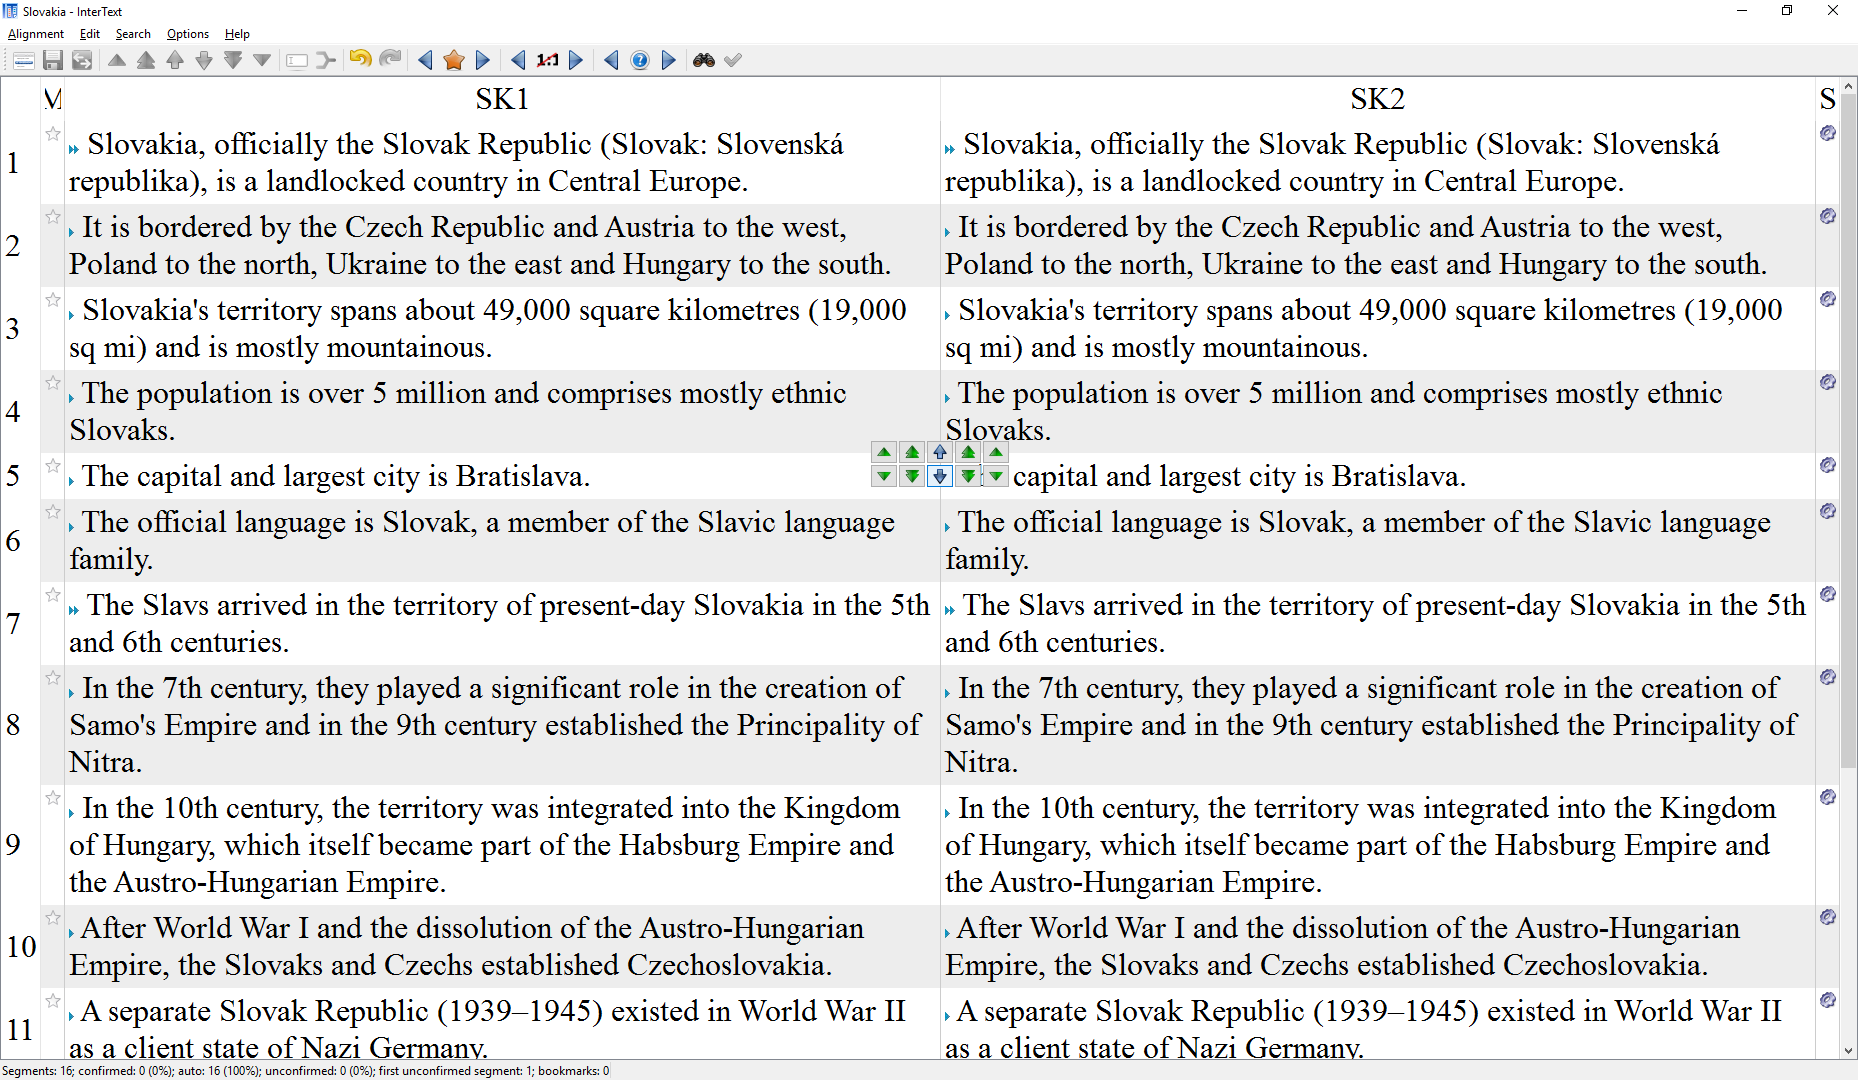
\includegraphics[scale=0.33]{intertext_interface}\end{center}
	\caption[Aplikácia InterText]{Aplikácia InterText}\label{fig:intertext_interface}
\end{figure}

%
% NOVA Text Aligner
%
\ifthenelse {\boolean{bachelor}}
{
	%\subsection{Subsection}
	\subsection{NOVA Text Aligner}
}
{
	%\section{Subsection}
	\section{NOVA Text Aligner}
}
NOVA Text Aligner\footnote{http://www.supernova-soft.com/wpsite/products/text-aligner/} je aplikácia na zarovnávanie textu, pričom nevyužíva algoritmy na zarovnávanie textu, ale používateľ si musí sám určiť zarovnanie.

Ako vidno na obrázku~\fullref{fig:nova_text_aligner_interface} hlavná editovacia časť aplikácie je rozdelená do dvoch častí. Umožňuje do ľavej aj pravej časti načítať rôzny text, v ktorom sa dá veľmi jednoducho vyhľadávať, k čomu napomáha zvýraznenie vyhľadaných slov. Načítaný text je možné premiestňovať a zoskupovať, či už podľa riadkov alebo aj v celých blokoch a nechýba možnosť editovať text. Je možné si túto aplikáciu prispôsobiť. Ponúka možnosti ako zmena typu písma a pod. Finálny spracovaný text sa dá exportovať do viacerých formátov, z ktorých populárne sú formáty elektronických knižiek EPUB a MOBI.

Aplikácia je zameraná hlavne na usporadúvanie textu, nezaznamenáva si používateľove zmeny textu a neprispôsobuje sa podľa toho pri ďalšom použití a funguje iba lokálne. NOVA Text Aligner je dostupná iba v skúšobnej verzií, pre dlhodobé používanie si treba zakúpiť licenciu.

\begin{figure}[H]
	\begin{center}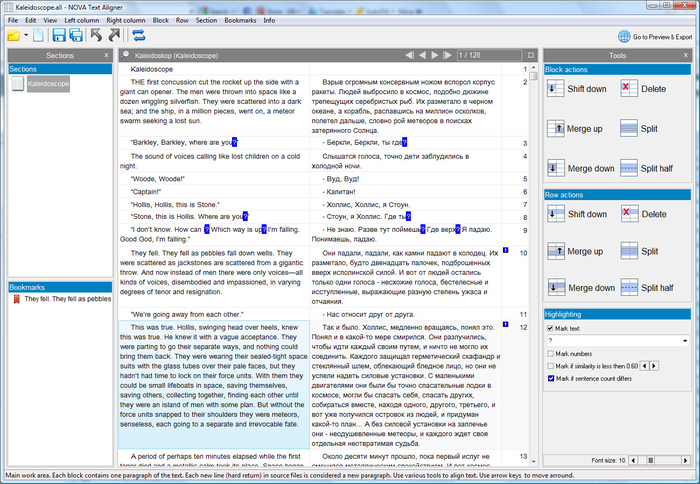
\includegraphics[scale=0.56]{nova_text_aligner_interface}\end{center}
	\caption[Aplikácia NOVA Text Aligner]{Aplikácia NOVA Text Aligner\footnotemark}\label{fig:nova_text_aligner_interface}
\end{figure}
\footnotetext{http://parallel-text-aligner.en.softonic.com/}

%
% LF Aligner
%
\ifthenelse {\boolean{bachelor}}
{
	%\subsection{Subsection}
	\subsection{LF Aligner}
}
{
	%\section{Subsection}
	\section{LF Aligner}
}
Aplikácia LF Aligner\footnote{www.sourceforge.net/projects/aligner} je zameraná na spracovanie textu rôznych jazykov. Ponúka možnosť použiť až 99 jazykov, čo ale znamená 99 vstupných súborov, každý so zvoleným jazykom. Dokáže spracovať rôzne typy vstupných súborov od čistého textu, PDF súborov, cez URL stránok s textom až po správy Európskeho parlamentu, ktoré automaticky stiahne. Výstup môže byť taktiež viacerých druhov, napríklad cez grafické rozhranie LF Aligner alebo vygenerovanie XLS súboru. Na obrázku~\fullref{fig:lf_aligner_interface} vidno grafické rozhranie tejto aplikácie, ktoré ponúka mnohé vymoženosti. Samozrejmosťou je možnosť premiestňovať a zoskupovať riadky, doplnenie ďalšieho súboru na spracovávanie, uloženie zmien súboru prepísaním jeho dát a mnohé ďalšie.

\begin{figure}[H]
	\begin{center}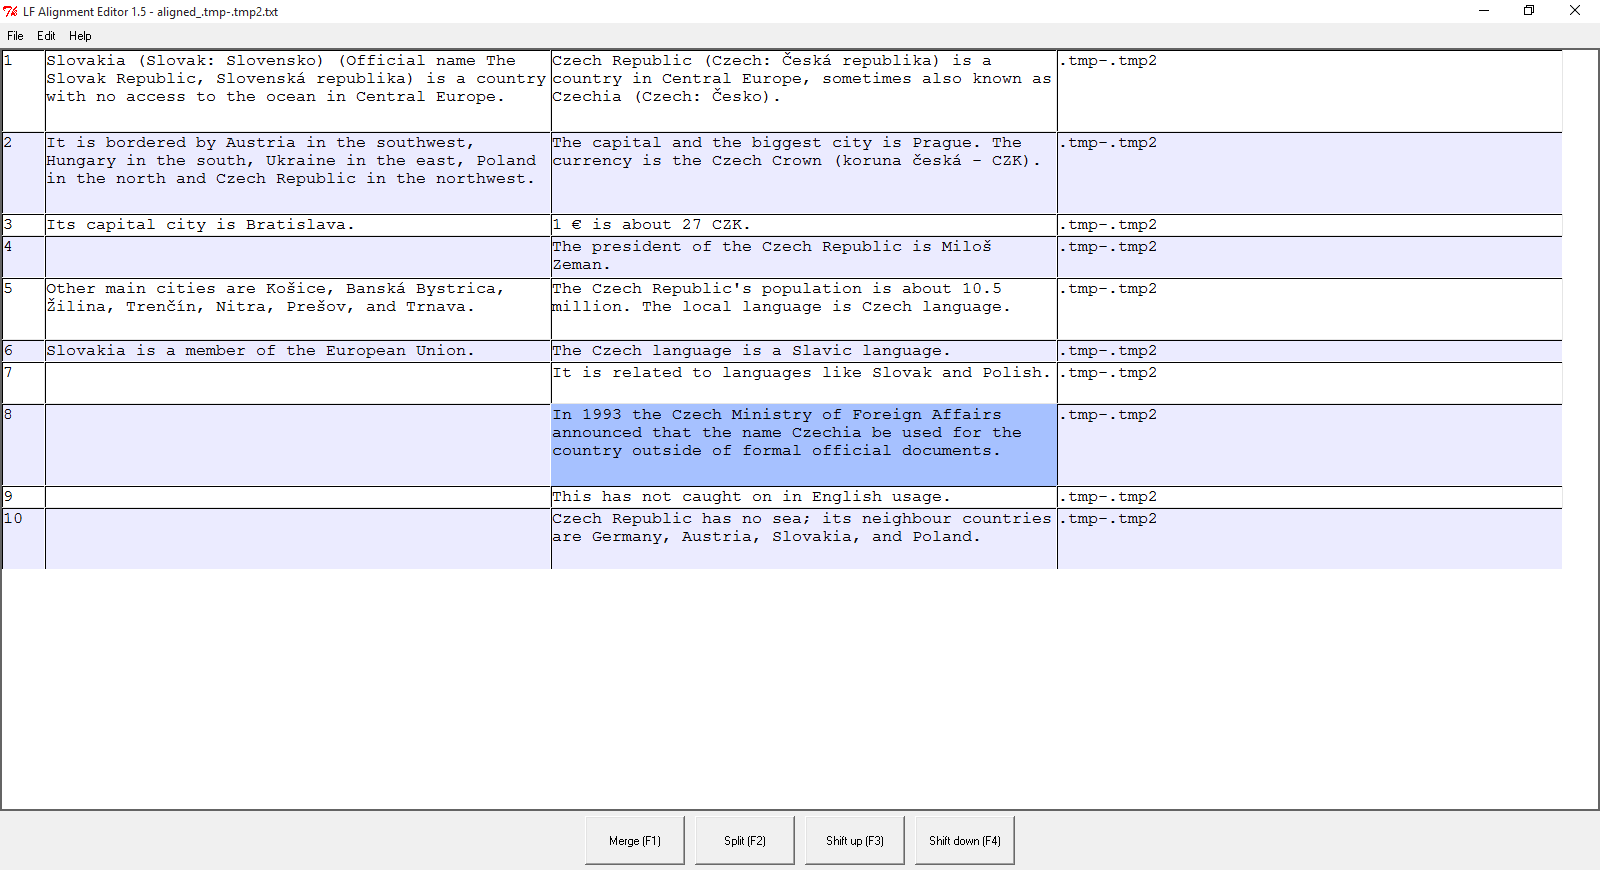
\includegraphics[scale=0.33]{lf_aligner_interface}\end{center}
	\caption[Aplikácia LF Aligner]{Aplikácia LF Aligner}\label{fig:lf_aligner_interface}
\end{figure}
\footnotetext{http://parallel-text-aligner.en.softonic.com/}

%
% Google Translate
%
\ifthenelse {\boolean{bachelor}}
{
	%\subsection{Subsection}
	\subsection{Google Translate}
}
{
	%\section{Subsection}
	\section{Google Translate}
}
Za najznámejšieho zástupcu webových nástrojov na spracovanie paralelných textov sa dá pokladať nástroj Google Translate\footnote{translate.google.com}. Využíva sa na preklad slov, viet, ale dokáže spracovať aj celé texty. Momentálne podporuje preklad z a do 91 jazykov. Dokáže rozpoznať a preložiť hovorenú reč aj písaný text. Pri preklade jednotlivých slov zobrazuje viacero možných prekladov do druhého jazyka, pričom pri preklade z anglického jazyka ponúka aj ukážky viet, v ktorých sa prekladané slovo môže použiť. Správnu výslovnosť preloženého aj prekladaného slova alebo textu, si používateľ môže vypočuť na krátkej zvukovej ukážke.

Na obrázku~\fullref{fig:google_translate_example} je zobrazený preklad anglického textu do slovenského. Vidno, že preklad do minoritných jazykov ešte nie je dokonalý.

\begin{figure}[H]
	\begin{center}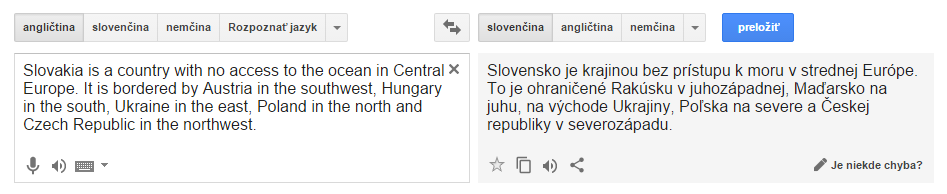
\includegraphics[scale=0.55]{google_translate_example}\end{center}
	\caption[Google Translate]{Google Translate}\label{fig:google_translate_example}
\end{figure}

%
% Zhrnutie aplikácií na spracovanie prirodzeného jazyka
%
\ifthenelse {\boolean{bachelor}}
{
	%\subsection{Subsection}
	\subsection{Zhrnutie}
}
{
	%\section{Subsection}
	\section{Zhrnutie}
}
\label{subsection:analysis2:zhrnutie}
Analyzovali sme aplikácie, ktoré umožňujú spravovať a editovať paralelný text. Za ich pomoci dokážeme zo vstupného textu získať výstupný text. Napríklad pri preklade máme vstupný text množinu viet v anglickom jazyku, ktorú chceme preložiť do slovenského jazyka a výstupný text je preloženú množinu viet. Pri zjednodušovaní textu je na vstupe taktiež množina viet a na výstupe je každá veta zo vstupnej množiny zjednodušená podľa istých pravidiel. Výstupný text vzniká určitou transformáciou vstupného textu, aplikovaním transformácie na každú vetu zdrojového textu.

Analyzované nástroje nespĺňajú všetky požiadavky na systém schopný spoznámkovať učebný text v takom rozsahu, ktorý by umožňoval používateľovi prispôsobiť si spracovaný text. Systém musí umožňovať editáciu jednotlivých viet výstupného textu podľa vôle používateľa. Tieto úpravy musí zohľadniť pri následnej aplikácií transformácií vstupného textu. Dáta ohľadne spoznámkovávania textu musia byť uložené na externom úložisku, ako napríklad v databáze na serveri.
